\section{Random Matrices}

This chapter mostly focuses on the theory regarding random matrices - nets, covering and packing numbers. 
Applications include community detection, covariance estimation, and spectral clustering.



% ----------4.1----------
\subsection{A Quick Refresher on Linear Algebra}

\subsubsection{Singular Value Decomposition}
\begin{theorem}[SVD]
\label{thm:4.1.1}
Any $m \times n$ matrix $A$ with real entries can be written as 
\[ A = \sum_{i = 1}^{r} \sigma_i u_i v_i^T \text{ where } r = \min_{}(m, n). \]
Here $\sigma_i > 0$ are the \underline{singular values} of $A$, $u_I \in \mathbb{R}^m$ are orthonormal vectors 
called the \underline{left singular vectors} of $A$, and $v_i \in \mathbb{R}^n$ are orthonormal vectors called 
the \underline{right singular vectors} of $A$.
\end{theorem}

\begin{proof}
WLOG, we can assume that $m \geq n$ or else we can just take the transpose. Since $A^T A \in \mathbb{R}^
{n \times n}$ is a symmetric positive semidefinite matrix, the spectral theorem tells us that its eigenvalues 
are $\sigma_1^2, \dots, \sigma_n^2$ and corresponding orthonormal eigenvectors $v_1, \dots, v_n \in 
\mathbb{R}^n$, so that $A^T A v_i = \sigma_i^2 v_i$. The vectors $Av_i$ are orthogonal: 
\[ \left\langle Av_i, Av_j \right\rangle = \left\langle A^TA v_i, v_j \right\rangle 
= \sigma_i^2 \left\langle v_i, v_j \right\rangle = \sigma_i^2 \delta{ij}. \]
Therefore, there exist orthonormal vectors $u_1, \dots, u_n \in \mathbb{R}^n$ such that 
\[ Av_i = \sigma_i u_i, \quad i = 1, \dots, n. \]
For the above, for all $i$ with $\sigma_i \neq 0$, the vectors $u_i$ are uniquely defined and ensures that 
they are orthonormal. If $\sigma_i = 0$, then $Av_i = 0$ holds triviall. In this case, we can pick any $u_i$ 
while keeping orthonormality.

Since $v_1, \dots, v_n$ form an orthonormal basis of $\mathbb{R}^n$, we can write $I_n = \sum_{i = 1}^{n} 
v_i v_i^T$. Multiplying by $A$ on the left and plugging the equation above gives 
\[ A = \sum_{i = 1}^{n} (Av_i)v_i^T = \sum_{i = 1}^{n} \sigma_i u_i v_i^T. \]
\end{proof}

\begin{remark}[Geometric interpretation]
\label{rmk:4.1.2}
SVD gives a geometric view of matrices: it stretches the orthogonal direction of $v_i$ by $\sigma_i$, then 
rotates the space, mapping the orthonormal basis $v_i$ to $u_i$.
\end{remark}

\begin{remark}[SVD matrix form]
\label{rmk:4.1.3}
We can set $\sigma_i = 0$ for $i > r$ and arrange them in weakly decreasing order. Then by extending 
$\{u_i\}$ and $\{v_i\}$ to orthonormal bases in $\mathbb{R}^m$ and $\mathbb{R}^n$, we get 
\[ A = U \Sigma V^T \]
where $U$ is the $m \times m$ matrix with left singular vectors $u_i$ as columns, $V$ is the $n \times n$ 
orthogonal matrix with right singular vectors $v_i$ as columns, and $\Sigma$ is the $m \times n$ diagonal 
matrix with the singular values $\sigma_i$ on the diagonal. If $A$ is symmetric, we get the spectral 
decomposition instead: 
\[ A = U \Lambda U^T. \]
\end{remark}

\begin{remark}[Spectral decomposition v.s. SVD]
\label{rmk:4.1.4}
The spectral and singular value decompositions are tightly connected. Since 
\[ AA^T = \sum_{i = 1}^{r} \sigma_i^2 u_i u_i^T \text{ and } A^T A = \sum_{i = 1}^{r} \sigma_i^2 v_i v_i^T \]
the left singular vectors $u_i$ of $A$ are the eigenvectors of $AA^T$, while the right singular vectors $v_i$ 
of $A$ are the eigenvectors of $A^T A$, and the singular values $\sigma_i$ of $A$ are 
\[ \sigma_i(A) = \sqrt{\lambda_i(AA^T)} = \sqrt{\lambda_i(A^T A)}. \]
\end{remark}

\begin{remark}[Orthogonal projection]
\label{rmk:4.1.5}
Consider the orthogonal projection $P$ in $\mathbb{R}^n$ onto a $k$-dimensional subspace $E$. The projection 
of a vector $x$ onto $E$ is given by $Px = \sum_{i = 1}^{k} \left\langle u_i, x \right\rangle u_i$ where 
$u_1, \dots, u_k$ is an orthonormal basis of $E$. We can rewrite this as 
\[ P = \sum_{i = 1}^{k} u_i u_i^T = UU^T \]
where $U$ is the $n \times k$ matrix with orthonormal columns $u_i$. In particular, $P$ is a symmetric 
matrix with eigenvalues $\underbrace{1, \dots, 1}_{k}, \underbrace{0, \dots, 0}_{n - k}$.
\end{remark}

\subsubsection{Min-max Theorem}
\label{thm:4.1.6}
There is another optimization-based description of eigenvalues:
\begin{theorem}[Min-max theorem for eigenvalues]
The $k$-th largest eigenvalue of an $n \times n$ symmetric matrix $A$ can be written as 
\[ \lambda_k(A)= \max_{\dim{E} = k} \min_{x \in S(E)} x^T Ax 
= \min_{\dim{E} = n-k+1} \max_{x \in S(E)} x^T Ax, \]
where the first max/min is taking with respect to all subspaces of a fixed dimension, and $S(E)$ denotes 
the Euclidean unit sphere of $E$, i.e. the set of all unit vectors in $E$. 
\end{theorem}

\begin{proof}
Let us focus on the first equation. To prove the upper bound on $\lambda_k$, we need to find a $k$-dimensional 
subspace $E$ such that 
\[ x^T Ax \geq \lambda_k \text{ for all } x \in S(E). \]
To find the set $E$, take the spectral decomposition $A = \sum_{i = 1}^{n} \lambda_i u_i u_i^T$ and pick the 
subspace $E = \mathrm{span}(u_1, \dots, u_k)$. The eigenvectors form an orthonormal basis of $E$, so any vector 
$x \in S(E)$ can be written as $x = \sum_{i = 1}^{k} a_i u_i$. Then by orthonormality of $u_i$ and 
monotonicity of $\lambda_i$, we get 
\[ x^T Ax = \sum_{i = 1}^{k} \lambda_i a_i^2 \leq \lambda_k \sum_{i = 1}^{k} a_i^2 = \lambda_k \]
and we have the upper bound. For the lower bound on $\lambda_k$, we need to find $x \in S(E)$ such that 
$x^T Ax \leq \lambda_k$. Here we let the subspace be $F = \mathrm{span}(u_k, \dots, u_n)$. 

Since $\dim{E} + \dim{F} = n + 1$, the intersection of $E$ and $F$ is nontrivial hence there is a unit 
vector $x \in E \cap F$.  Writing $x = \sum_{i = k}^{n} a_i u_i$, we get 
\[ x^T Ax = \sum_{i = k}^{n} \lambda_i a_i^2 \geq \lambda_k \sum_{i = k}^{n} a_i^2 = \lambda_k. \]
Then we get the lower bound, and hence the first equality is done.

The second equality is by applying the same technique to $-A$ and reversing the eigenvalues.
\end{proof}

Applying \cref{thm:4.1.6} to $A^T A$ and using \cref{rmk:4.1.4}, we get 
\begin{corollary}[Min-max theorem for singular values]
\label{cor:4.1.7}
Let $A \in \mathbb{R}^{m \times n}$ with singular values $\sigma_1 \geq \cdots \geq \sigma_n \geq 0$. Then 
\[ \sigma_k(A) = \max_{\dim{E} = k} \min_{x \in S(E)} \lVert Ax \rVert_{2} 
= \min_{\dim{E} = n-k+1} \max_{x \in S(E)} \lVert Ax \rVert_{2} \]
with the same notation as \cref{thm:4.1.6}.
\end{corollary}

\subsubsection{Frobenius and Operator Norms}
\begin{definition}[]
\label{def:4.1.8}
For a matrix $A \in \mathbb{R}^{m \times n}$, the \underline{Frobenius norm} is 
\[ \lVert A \rVert_{F} := \left( \sum_{i = 1}^{m} \sum_{j = 1}^{n} A_{ij}^2 \right)^{1/2}. \]

The \underline{operator norm} of $A$ is the smallest number $K$ such that 
\[ \lVert Ax \rVert_{2} \leq K \lVert x \rVert_{2} \text{ for all } x \in \mathbb{R}^n. \]
Equivalently, 
\[ \lVert A \rVert_{} = \max_{x \neq 0} \frac{\lVert Ax \rVert_{2}}{\lVert x \rVert_{2}} 
= \max_{\lVert x \rVert_{2} \leq 1} \lVert Ax \rVert_{2} 
= \max_{\lVert x \rVert_{2} = 1} \lVert Ax \rVert_{2} 
= \max_{\lVert x \rVert_{2} = \lVert y \rVert_{2} = 1} |y^T Ax|. \]
\end{definition}
From the Frobenius norm, we can get that 
\[ \left\langle A, B \right\rangle = \sum_{i = 1}^{m} \sum_{j = 1}^{n} A_{ij} B_{ij} = \mathrm{tr}(A^T B). \]
Also, from above we can get 
\[ \lVert A \rVert_{F}^2 = \left\langle A, A \right\rangle = \mathrm{tr}(A^T A). \]

For the operator norm, the first three equations follows by rescaling, and the last one comes from the 
duality formula: 
\[ \lVert Ax \rVert_{} = \max_{\lVert y \rVert_{2} = 1} \left\langle Ax, y \right\rangle. \]
Here the absolute sign does not matter.

\begin{remark}[Other operator norms]
\label{rmk:4.1.9}
We can replace the $\ell^2$ norm in \cref{def:4.1.8} with other norms to get a more general concept of 
operator norms (Exercise 4.18-4.22).
\end{remark}

\subsubsection{The Matrix Norms and the Spectrum}
\begin{lemma}[Orthogonal invariance]
\label{lem:4.1.10}
The Frobenius and spectral norms are orthogonal invariant, meaning that for any $A$ and orthogonal matrices 
$Q, R$ with proper dimensions, we have 
\[ \lVert QAR \rVert_{F} = \lVert A \rVert_{F} \text{ and } \lVert QAR \rVert_{} = \lVert A \rVert_{}. \]
\end{lemma}

\begin{proof}
For the Frobenius norm, by one of the formulas above, 
\begin{align*}
	\lVert QAR \rVert_{F} 
	&= \mathrm{tr}(R^T AT Q^T QAR) \\
	&= \mathrm{tr}(R^T A^T AR) \\
	&= \mathrm{tr}(RR^T A^T A) \\
	&= \mathrm{tr}(A^T A) \\
	&= \lVert A \rVert_{F}^2.
\end{align*}
For the spectral norm, by an equivalent characterization, $\lVert QAR \rVert_{}$ is obtained by maximizing the 
bilinear form $y^T QARx = (Qy)^T A (Rx)$ over all unit vectors $x, y$. Since $Q, R$ are orthogonal, 
$Qy$ and $Rx$ also range over all unit vectors, so we just get $\lVert A \rVert_{}$ as a result.
\end{proof}

\begin{lemma}[Matrix norms via singular values]
\label{lem:4.1.11}
For any $A \in \mathbb{R}^{m \times n}$ with singular values $\sigma_1 \geq \cdots \geq \sigma_n$, 
\[ \lVert A \rVert_{F} = \left( \sum_{i = 1}^{n} \sigma_i^2 \right)^{1/2} \text{ and } 
\lVert A \rVert_{} = \sigma_1. \]
\end{lemma}

\begin{proof}
For the Frobenius norm, by orthogonal invariance (\cref{lem:4.1.10}), 
\[ \lVert A \rVert_{F} = \lVert U \Sigma V^T \rVert_{F} = \lVert \Sigma \rVert_{F} \]
which directly gives us the result.

The result for the operator norm directly follows from \cref{cor:4.1.7} with $k = 1$.
\end{proof}

\begin{remark}[Symmetric matrices]
\label{rmk:4.1.12}
For a symmetric matrix $A$ with eigenvalues $\lambda_k$, 
\[ \lVert A \rVert_{} = \max_{k}|\lambda_k| = \max_{\lVert x \rVert_{} = 1} |x^T Ax|. \] 
The first equality becomes \cref{lem:4.1.11} since the singular values of $A$ are $|\lambda_k|$. The 
min-max theorem (\cref{thm:4.1.6}) gives $|\lambda_k| \leq \max_{\lVert x \rVert_{} = 1} |x^T Ax|$, proving 
the upper bound in the equation above. The lower bound can be proven by taking $x - y$ in the definition of 
the operator norm (\cref{def:4.1.8}).
\end{remark}

\subsubsection{Low-rank Approximation}
For a given matrix $A$, what is the closest approximation to it for a given matrix of rank $k$? The answer 
is just truncating the SVD of A: 

\begin{theorem}[Eckart-Young-Mirski theorem]
\label{thm:4.1.13}
Let $A = \sum_{i = 1}^{n} \sigma_i u_i v_i^T$. Then for any $1 \leq k \leq n$,
\[ \min_{\mathrm{rank}(B) = k} \lVert A - B \rVert_{} = \sigma_{k + 1}. \]
The minimum is attained at $B = \sum_{i = 1}^{k} \sigma_i u_i v_i^T$.
\end{theorem}

\begin{proof}
If $B \in \mathbb{R}^{m \times n}$ has rank $k$, $\dim{\ker{(B)}} = n - k$. Then the min-max theorem 
(\cref{cor:4.1.7}) for $k + 1$ instead of $k$ gives 
\[ \lVert A - b \rVert_{} \geq \max_{x \in S(E)} \lVert (A - B)x \rVert_{2} 
= \max_{x \in S(E)} \lVert Ax \rVert_{2} \geq \sigma_{k + 1}. \]

In the opposite direction, setting $B = \sum_{i = 1}^{k} \sigma_i u_i v_i^T$ gives $A - b = 
\sum_{i = k + 1}^{n} \sigma_i u_I v_i^T$. The maximal singular value of this matrix $\sigma_{k + 1}$, 
which is the same as its operator norm by \cref{lem:4.1.11}.
\end{proof}

\subsubsection{Perturbation Theory}
We can also study how eigenvalues/eigenvectors change under matrix perturbations: 
\begin{lemma}[Weyl inequality]
\label{lem:4.1.14}
The $k$-th largest eigenvalue of symmetric matrices $A, B$ satisfy 
\[ |\lambda_k(A) - \lambda_k(B)| \leq \lVert A - B \rVert_{}. \]
Similarly, the $k$-th largest singular values of general rectangular matrices satisfy 
\[ |\sigma_k(A) - \sigma_k(B)| \leq \lVert A - B \rVert_{}. \]
\end{lemma}

A similar result holds for eigenvectors, however we have to track the same eigenvector before and after the 
perturbation. If the eigenvalues are too close, a small perturbation can swap them, leading to huge error 
since their eigenvectors are orthogonal and far apart.

\begin{theorem}[Davis-Kahan inequality]
\label{thm:4.1.15}
Consider two symmetric matrices $A, B$ with spectral decompositions 
\[ A = \sum_{i = 1}^{n} \lambda_i u_i u_i^T, \ B = \sum_{i = 1}^{n} \mu_i v_i v_i^T, \]
where the eigenvalues are weakly decreasing. Assume the the $k$-th largest eigenvalue of $A$ is 
$\delta$-seperated from the rest: 
\[ \min_{i \neq k} |\lambda_k - \lambda_i| = \delta > 0. \]
Then the angle between the eigenvectors $u_k$ and $v_k$ satisfies
\[ \sin{\angle u_k, v_k} \leq \frac{2 \lVert A - B \rVert_{}}{\delta}. \]
\end{theorem}

The theorem above can be derived via a stronger result of Davis-Kahan focusing on spectral projections - 
the orthogonal projections onto the span of some subset of eigenvectors:

\begin{lemma}[Davis-Kahan inequality for spectral projections]
\label{lem:4.1.16}
Consider $A, B$ as in \cref{thm:4.1.15}. Let $I, J$ be two $\delta$-seperated subsets of $\mathbb{R}$, with 
$I$ being an interval. Then the spectral projections 
\[ P = \sum_{i: \lambda_i \in I}^{} u_i u_i^T \text{ and } 
Q = \sum_{j: \lambda_j \in J}^{} v_j v_j^T \text{ satisfy } \lVert QP \rVert_{} 
\leq \frac{\lVert A - B \rVert_{}}{\delta}. \]
\end{lemma}

\begin{proof}
WLOG, assume $I$ is finite and closed. Adding the same multiple of Identity to $A$ and $B$, we can center 
$I$ as $[-r, r]$, so that $|\lambda_i| \leq r$ for $i \in I$ and $|\mu_j| \geq r + \delta$ for $\mu_j \in J$. 
The idea is to see how $P$ and $Q$ interact through $H := B - A$:
\[ \lVert H \rVert_{} \geq \lVert QHP \rVert_{} = \lVert QBP - QAP \rVert_{} 
\geq \lVert QBP \rVert_{} - \lVert QAP \rVert_{}. \]
The spectral projection $A$ commutes with $B$, hence 
\[ \lVert QBP \rVert_{} \geq \lVert BQP \rVert_{} \geq (r + \delta)\lVert QP \rVert_{}. \]
To see the last inequality, the image of $Q$ is spanned by orthogonal vectors $v_j$ with $|\mu_j| \geq 
r + \delta$. The matrix $B$ maps each such vector $v_j$ to $\mu_j v_j$, hence scaling it by at least 
$r + \delta$. Thus $B$ expands the norm of any vector in the image of $Q$ by at least $r + \delta$ so
\[  \lVert BQPx \rVert_{2} \geq (r + \delta)\lVert QPx \rVert_{2} \text{ for any } x. \]
Taking the supremum over all unit vectors gives the result with the operator norm. 

Also, $AP = PAP = \sum_{i: \lambda_i \in I}^{} \lambda_i u_i u_i^T$ so 
\[ \lVert QAP \rVert_{} = \lVert QPAP \rVert_{} \leq \lVert QP \rVert_{} \cdot \lVert AP \rVert_{} 
\leq r \lVert AP \rVert_{}, \]
because $\lVert AP \rVert_{} = \max_{i: \lambda_i \in I} |\lambda_i| \leq r$. Putting the two bounds together 
we get 
\[ \lVert H \rVert_{} = \lVert B - A \rVert_{} \geq \delta \lVert QP \rVert_{}, \]
which completes the proof.
\end{proof}

\begin{proof}[Proof for \cref{thm:4.1.15}]
Since the LHS is a trig angle, we can assume that $\varepsilon := \lVert A - B \rVert_{} \leq \delta / 2$ or 
else the inequality holds trivially. By Weyl inequality (\cref{lem:4.1.14}), $|\lambda_j - \mu_j| 
\leq \varepsilon$ for each $j$ hence 
\[ \min_{j: j \neq k} |\lambda_k - \mu_k| \geq \min_{j: j \neq k} |\lambda_k - \lambda_j| - \varepsilon 
= \delta - \varepsilon \geq \delta/2. \]
Apply \cref{lem:4.1.16} for the $\delta/2$-seperated subsets $I = \{\lambda_k\}$ and $J = \{\mu_j: 
j \neq k\}$ to get $\lVert QP \rVert_{} \leq 2 \varepsilon / \delta$. 

Since $P$ and $I_n - Q$ are the orthogonal projections on the directions of $u_k$ and $v_k$ respectively, 
\[ \lVert QP \rVert_{} = \max_{\lVert x \rVert_{} = 1} \lVert QPx \rVert_{2} 
= \lVert Q u_k \rVert_{2} = \sin{\angle(u_k, v_k)}. \]
Combining this with the inequality on $\lVert QP \rVert_{}$ above completes the proof.
\end{proof}

\subsubsection{Isometries}
The singular values of a matrix $A$ satisfy (by the min-max theorem)
\[ \sigma_n \lVert x - y \rVert_{2} \leq \lVert Ax - Ay \rVert_{2} \leq \sigma_1 \lVert x - y \rVert_{2}. \]
The extreme singular values set the limits on how the linear map $A$ distorts space.

A matris is an \underline{isometry} if 
\[ \lVert Ax \rVert_{2} = \lVert x \rVert_{2} \text{ for all } x \in \mathbb{R}^n. \]
Notice that $A$ need not be a square matrix. T

For $A \in \mathbb{R}^{m \times n}$ with $m \geq n$, the following are equivalent: 
\begin{enumerate}
	\item The columns of $A$ are orthonormal, i.e. $A^T A = I_n$, 
	\item A is an isometry, 
	\item All singular values of $A$ are 1.
\end{enumerate}

There is a stronger result where the properties hold approximately instead of exactly (useful when 
dealing with random matrices): 
\begin{lemma}[Approximate isometries]
\label{lem:4.1.17}
Let $A \in \mathbb{R}^{m \times n}$ with $m \geq n$ and let $\varepsilon \geq 0$. The following are equivalent: 
\begin{enumerate}
	\item $\lVert A^T A - I_n \rVert_{} \leq \varepsilon$.
	\item $(1 - \varepsilon)\lVert x \rVert_{2}^2 \leq \lVert Ax \rVert_{2}^2 \leq 
	(1 + \varepsilon)\lVert x \rVert_{2}^2$ for any $x \in \mathbb{R}^n$.
	\item $1 - \varepsilon \leq \sigma_n^2 \leq \sigma_1^2 \leq 1 + \varepsilon$.
\end{enumerate}
\end{lemma}

\begin{proof}
(a) $\Leftrightarrow$ (b) By rescaling, we can assume that $\lVert x \rVert_{2} = 1$ in (b). Then we have 
\[ \lVert A^T A - I_n \rVert_{} = \max_{\lVert x \rVert_{2} = 1} 
|x^T (A^T A - I_n)x| = \max_{\lVert x \rVert_{2} = 1} |\lVert Ax \rVert_{2}^2 - 1|, \]
The above being bounded by $\varepsilon$ is equivalent to (b) for all unit vectors $x$.

(b) $\Leftrightarrow$ (c) follows from the relationship for singular values distorting space from above.
\end{proof}

\begin{remark}[]
\label{rmk:4.1.18}
Here is a more handy version of (a) $\Rightarrow$ (c) in \cref{lem:4.1.17}. For $z \in \mathbb{R}$ and 
$\delta \geq 0$, 
\[ |z^2 - 1| \leq \max_{}(\delta, \delta^2) \implies |z - 1| \leq \delta. \]
Then substituting $\varepsilon = \max_{}(\delta, \delta^2)$, we get 
\[ \lVert A^T A - I_n \rVert_{} \leq \max_{}(\delta, \delta^2)  
\implies 1 - \delta \leq \sigma_n \leq \sigma_1 \leq 1 + \delta. \]
\end{remark}



% ----------4.2----------
\subsection{Nets, Covering, and Packing}
The $\varepsilon$-net argument is useful for analysis of random matrices. It is also connected to ideas like 
covering, packing, entropy, volume, and coding.

\begin{definition}[]
\label{def:4.2.1}
Let $(T, d)$ be a metric space. Consider $K \subset T$ and $\varepsilon > 0$. A subset $\mathcal{N} \subset 
T$ is called an \underline{$\varepsilon$-net} of $K$ is every point in $K$ is within distance $\varepsilon$ 
of some point in $\mathcal{N}$, i.e.
\[ \forall x \in K \exists x_0 \in \mathcal{N}: \ d(x, x_0) \leq \varepsilon. \]
Equivalently, $\mathcal{N}$ is an $\varepsilon$-net of $K$ if the balls of radius $\varepsilon$ centered at 
points in $\mathcal{N}$ cover $K$, like in the figure below:

\begin{center}
	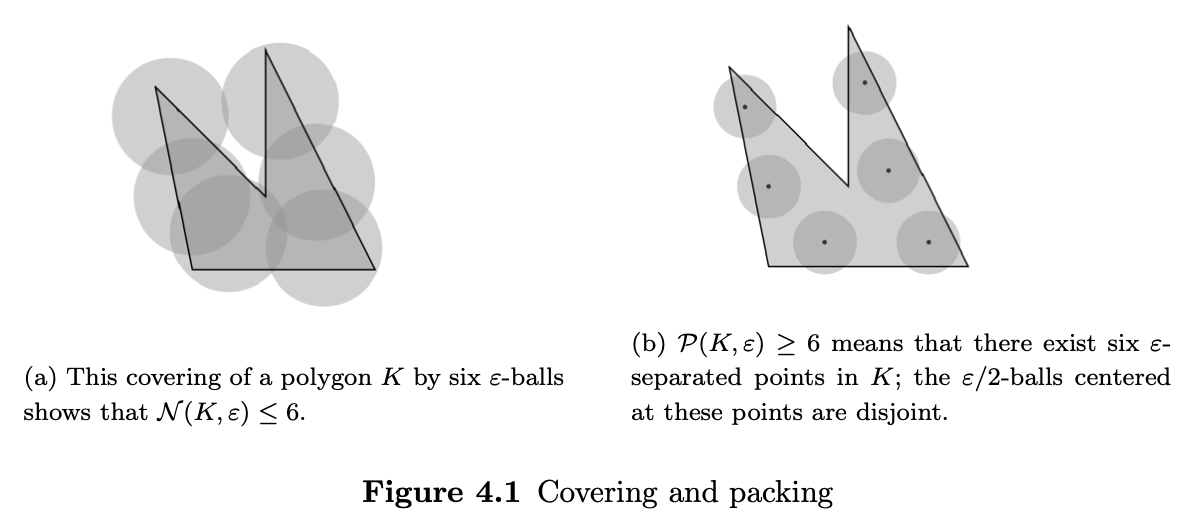
\includegraphics[width=0.8\textwidth]{Chapter 4/fig4-1.png}
\end{center}
\end{definition}

\begin{definition}[]
\label{def:4.2.2}
The smallest cardinality of an $\varepsilon$-net of $K$ is called the \underline{covering number} of 
$K$, and is denoted $\mathcal{N}(K, d, \varepsilon)$.
\end{definition}

\begin{remark}[Compactness]
\label{rmk:4.2.3}
An important result in real analysis says that a subset $K$ of a complete metric space $(T, d)$ is 
\underline{precompact} (i.e. the closure of $K$ is compact) if and only if
\[ N(K, d, \varepsilon) < \infty \text{ for every } \varepsilon > 0. \]
We can think about the covering numbers as a quantitative measure of how compact $K$ is.
\end{remark}

\begin{definition}[]
\label{def:4.2.4}
A subset $\mathcal{N}$ of a metric space $(T, d)$ is \underline{$\varepsilon$-seperated} if 
\[ d(x, y) > \varepsilon \text{ for any distinct points } x, y \in \mathcal{N}. \]
The largest possible cardinality of an $\varepsilon$-seperated subset of a given $K \subset T$ is called 
the \underline{packing number} of $K$ and is denoted $\mathcal{P}(K, d, \varepsilon)$.
\end{definition}

\begin{remark}[Packing balls into $K$]
\label{rmk:4.2.5}
If $\mathcal{N}$ is $\varepsilon$-seperated, the closed $\varepsilon / 2$-balls centered at points in 
$\mathcal{N}$ are disjoint by the triangle inequality, hence we can always pack into $K$ at least 
$\mathcal{P}(K, d, \varepsilon)$ disjoint $\varepsilon / 2$-balls.
\end{remark}

\begin{lemma}[Nets from seperated sets]
\label{lem:4.2.6}
Let $\mathcal{N}$ be a maximal $\varepsilon$-seperated subset of $K$, i.e. adding any new point to $\mathcal{N}$ 
destroys the seperation property. Then $\mathcal{N}$ is an $\varepsilon$-net of $K$.
\end{lemma}

\begin{proof}
Let $x \in K$. We want to show that there exists $x_0 \in \mathcal{N}$ such that $d(x, x_0) \leq \varepsilon$. 
If $x \in \mathcal{N}$, the conclusion is trivial by choosing $x_0 = x$. Suppose $x \notin \mathcal{N}$. 
The maximality assumption implies that $\mathcal{N} \cup \{x\}$ is not $\varepsilon$-seperated, meaning 
$d(x, x_0) \leq \varepsilon$ for some $x_0 \in \mathcal{N}$.
\end{proof}

\begin{remark}[Constructing a net]
\label{rmk:4.2.7}
The lemma above (\cref{lem:4.2.6}) gives an iterative algorithm to construct an $\varepsilon$-net for a 
given set $K$. Pick $x_1 \in K$ arbitrarily, then pick $x_2 \in K$ that is farther than $\varepsilon$ from 
$x_1$, then pick $x_3$ that it is farther than $\varepsilon$ from both $x_1$ and $x_2$, and so on. If $K$ 
is compact, then the process will stop in a finite number of iterations!
\end{remark}

\begin{lemma}[Equivalence of covering and packing numbers]
\label{lem:4.2.8}
For any set $K \subset T$ and $\varepsilon > 0$, 
\[ \mathcal{P}(K, d, 2 \varepsilon) \leq \mathcal{N}(K, d, \varepsilon) 
\leq \mathcal{P}(K, d, \varepsilon). \]
\end{lemma}

\begin{proof}
The upper bound follows from \cref{lem:4.2.6} because the packing number is exactly the number that makes 
$\mathcal{N}$ a maximal $\varepsilon$-seperated set.

For the lower bound, take any $2 \varepsilon$-seperated subset $\mathcal{P} = \{x_i\}$ in $K$ and any 
$\varepsilon$-net $\mathcal{N} = \{y_j\}$ of $K$. By definition, each point $x_i$ is in the $\varepsilon$-ball 
centered at some point $y_j$. Since any closed $\varepsilon$ ball cannot contain two $2 \varepsilon$-seperated 
points, each $\varepsilon$-ball centered at $y_j$ can contain at most one $x_i$. The pigeonhole principle 
gives $|\mathcal{P}| \leq |\mathcal{N}|$. Since $\mathcal{P}$ and $\mathcal{N}$ are arbitrary, the bound follows.
\end{proof}

\subsubsection{Covering Numbers and Volume}
This sections is about covers with $T = \mathbb{R}^n$ with the Eudlidean metric 
\[ d(x, y) = \lVert x - y \rVert_{2}. \]
Therefore, we can omit the metric when denoting the covering and packing numbers: 
\[ \mathcal{N}(K, \varepsilon) = \mathcal{N}(K, d, \varepsilon). \]
How do the covering numbers relate to the most classical measure, the volume of $K$ in $\mathbb{R}^n$? 

\begin{definition}[Minkowski sum]
\label{def:4.2.9}
Let $A, B \subseteq \mathbb{R}^n$. The \underline{Minkowski sum} is defined as 
\[ A + B := \{ A + B: \ a \in A, b \in B \}. \]
Below is an example of the Minkowski sum of two sets on the plane:

\begin{center}
	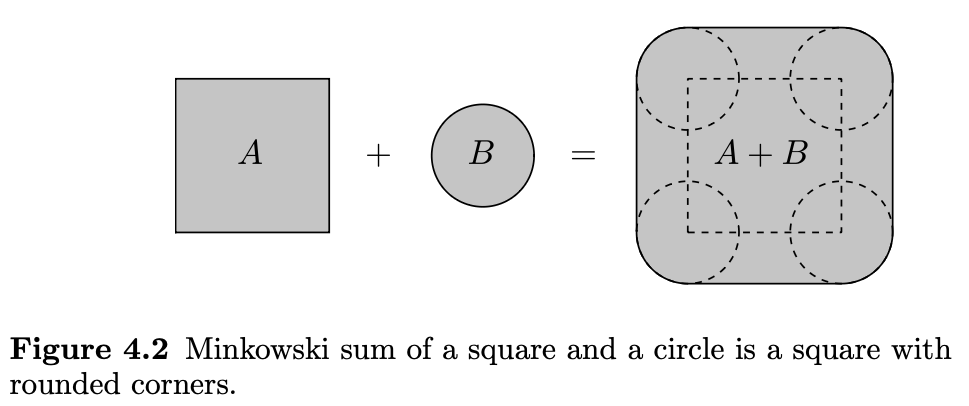
\includegraphics[width=0.8\textwidth]{Chapter 4/fig4-2.png}
\end{center}
\end{definition}

\begin{proposition}[Covering numbers and Volume]
\label{prop:4.2.10}
Let $K \subset \mathbb{R}^n$ and $\varepsilon > 0$. Then
\[ \frac{\mathrm{Vol}(K)}{\mathrm{Vol}(\varepsilon B_2^n)} \leq \mathcal{N}(K, \varepsilon) 
\leq \mathcal{P}(K, \varepsilon) \leq 
\frac{\mathrm{Vol}(K + (\varepsilon / 2)B_2^n)}{\mathrm{Vol}((\varepsilon / 2)B_2^n)}, \]
where $B_2^n$ denotes the unit ball in $\mathbb{R}^n$. 
\end{proposition}

\begin{proof}
The middle inequality was already proven in \cref{lem:4.2.8}, hence we focus on the left and right bounds.

(\textbf{Lower bound}) Let $N := \mathcal{N}(K, \varepsilon)$. Then $K$ can be covered by $N$ balls with radii 
$\varepsilon$. Comparing the volumes,
\[ \mathrm{Vol}(K) \leq N \cdot \mathrm{Vol}(\varepsilon B_2^n), \]
which gives the lower bound.

(\textbf{Upper bound}) Let $N := \mathcal{P}(K, \varepsilon)$. Then we can find $N$ disjoint closed 
$\varepsilon / 2$-balls with centers $x_i \in K$. While these balls may not fit entirely in $K$ (Figure 4-1), 
they do fit in a slightly inflated set, namely $K + (\varepsilon / 2)B_2^n$ (Basically putting balls at the 
boundary of $K$). Comparing the volume gives 
\[ N \cdot \mathrm{Vol}((\varepsilon / 2)B_2^n) \leq \mathrm{Vol}(K + (\varepsilon / 2)B_2^n), \]
which completes the upper bound.
\end{proof}

An important consequence of the volumetric bound is that the covering (hence packing) numbers are typically 
\textit{exponential} in the dimension $n$: 
\begin{corollary}[Covering numbers of the Euclidean ball]
\label{cor:4.2.11}
The covering numbers of the unit Euclidean ball $B_2^n$ satisfy the following for any $\varepsilon > 0$: 
\[ \left( \frac{1}{\varepsilon} \right)^n \leq \mathcal{N}(B_2^n, \varepsilon) 
\leq \left( \frac{2}{\varepsilon} + 1 \right)^n. \]
\end{corollary}

\begin{proof}
The lower bound immediately follows from \cref{prop:4.2.10}, since the volumd in $\mathbb{R}^n$ scale as 
$\mathrm{Vol}(\varepsilon B_2^n) = \varepsilon^n \mathrm{Vol}(B_2^n)$.

The upper bound follows from \cref{prop:4.2.10} as well:
\[ \mathcal{N}(B_2^n, \varepsilon) \leq 
\frac{\mathrm{Vol}((1 + \varepsilon / 2)B_2^n)}{\mathrm{Vol}((\varepsilon / 2)B_2^n)} 
= \frac{(1 + \varepsilon / 2)^n}{(\varepsilon / 2)^n} 
= \left( \frac{2}{\varepsilon} + 1 \right)^n. \]
\end{proof}

To simplify \cref{cor:4.2.11}, we can divide this into two cases for $\varepsilon$:

For $\varepsilon \in (0, 1]$, we have 
\[ \left( \frac{1}{\varepsilon} \right)^n \leq \mathcal{N}(B_2^n, \varepsilon) 
\leq \left( \frac{3}{\varepsilon} \right)^n. \]
In the other case where $\varepsilon > 1$, one $\varepsilon$-ball covers the unit ball hence 
$\mathcal{N}(B_2^n, \varepsilon) = 1$.

\begin{remark}[Volume of the ball]
\label{rmk:4.2.12}
The proof of \cref{cor:4.2.11} works with the volume of the Euclidean ball but never actually calculates it!
We can compute the volume geometrically, probabilistically, and analytically (Exercises 4.27-4.29), and 
also extend this notion of volume to $\ell^p$ balls (Exercise 4.30).
\end{remark}

\begin{remark}[How to construct a net?]
\label{rmk:4.2.13}
We have an algorithm to construct nets already (\cref{rmk:4.2.7}), but for the Euclidean ball, we can also 
use a scaled integer lattice (Exercise 4.31), or just use random points (Exercise 4.39).
\end{remark}

We can also use covering/packing notions for other objects via volumetric arguments, here is another example:

\begin{definition}[]
\label{def:4.2.14} 
The Hamming cube $\{0, 1\}^n$ consists of all binary strings of length $n$. To turn it into a metric space, 
we define the \underline{hamming distance} as the number of bits where the strings $x$ and $y$ differ:
\[ d_H(x, y) := |\{i: \ x(i) \neq y(i) \}|, \ x, y \in \{0, 1\}^n. \]
\end{definition}

\begin{proposition}[Covering and packing numbers of the Hamming cube]
\label{prop:4.2.15}
The covering and packing numbers of the Hamming cube $K = \{0, 1\}^n$ satisfy the following for any integer 
$m \in \{0, \dots, n\}$: 
\[ \frac{2^n}{\sum_{k = 0}^{m} \binom{n}{k}} \leq \mathcal{N}(K, d_H, m) 
\leq \mathcal{P}(K, d_H, m) \leq \frac{2^n}{\sum_{k = 0}^{\left\lfloor m/2 \right\rfloor} \binom{n}{k}}. \]
\end{proposition}

\begin{proof}
Use the volumetric argument from above using cardinality instead of the volume (Exercise 4.32).
\end{proof}



% ----------4.3----------
\subsection{Application: Error Correcting Codes}
Covering and packing arguments frequently appear in applications in \textit{coding theory}. We'll give two 
examples below.


\subsubsection{Metric Entropy and Complexity}
Intuitively, the covering and packing numbers measure the \textit{complexity} of a set $K$. Now we'll look at 
another concept related to that: The logarithm of the covering numbers $\log_{2}{\mathcal{N}(K, \varepsilon)}$ 
is often called the \textit{metric entropy} of the set $K$. 

\begin{proposition}[Metric entropy and coding]
\label{prop:4.3.1}
Let $(T, d)$ be a metric space, and consider a subset $K \subset T$. Let $\mathcal{C}(K, d, \varepsilon)$ denote 
the smallest number of bits sufficient to specify every point $x \in K$ with accuracy $\varepsilon$ in the 
metric $d$. Then 
\[ \log_{2}{\mathcal{N}(K, d, \varepsilon)} \leq \mathcal{C}(K, d, \varepsilon) 
\leq \left\lfloor \log_{2}{\mathcal{N}(K, d, \varepsilon/2)} \right\rfloor. \]
\end{proposition}

\begin{proof}
\textbf{(Lower bound)} Assume $\mathcal{C}(K, d, \varepsilon) \leq N$. This means that there exists a mapping 
(``encoding") of points $x \in K$ into bit strings of length $N$, which specifies every point with accuracy 
$\varepsilon$. This gives a partition of the domain $K$ into at most $2^N$ subsets, each consisting of the 
points represented by the same string (Figure 4.3). Each subset has diameter at most $\varepsilon$, so it can be 
comvered by a a ball centered in $K$ and with radius $\varepsilon$. Therefore, $K$ can be covered by at most 
$2^N$ balls with radius $\varepsilon$, meaning $\mathcal{N}(K, d, \varepsilon) \leq 2^N$. Taking logarithms 
gives the lower bound.

\begin{center}
    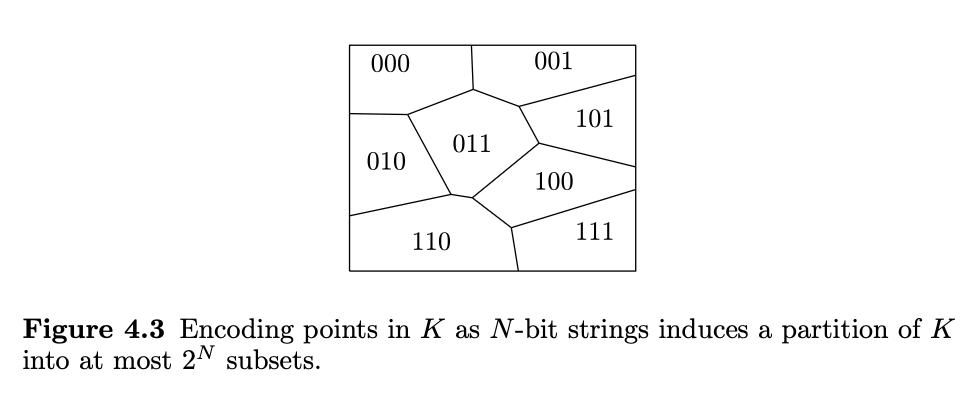
\includegraphics[width=0.8\textwidth]{Chapter 4/fig4-3.png}
\end{center}

\textbf{(Upper bound)} Assume $\log_{2}{\mathcal{N}(K, d, \varepsilon/2)} \leq N$ for some integer $N$. This 
means that there exists an $(\varepsilon/2)$-net $\mathcal{N}$ of $K$ with at most $w^N$ points. For each point 
$x \in K$, assign a closest point $x_0 \in \mathcal{N}$. Since there are at most $2^N$ such points, $N$ bits are 
sufficient to specify $x_0$. Let's show that the encoding $x \mapsto x_0$ represents points in $K$ with 
arbitrary accuracy $\varepsilon$. If both $x$ and $y$ are encoded by the same $x_0$ then by the triangle 
inequality, 
\[ d(x, y) \leq d(x, x_0) + d(x_0, y) \leq \frac{\varepsilon}{2} + \frac{\varepsilon}{2} = \varepsilon. \]
This shows that $\mathcal{C}(K, d, \varepsilon) \leq N$, which completes the proof.
\end{proof}


\subsubsection{Error Correcting Codes}
Suppose Alice wants to send to Bob a message with $k$ letters, e.g.
\[ x := \text{``fill the glass"}. \]
Suppose further that an adversary can corrupt Alice's message by changing up to $r$ letters. For example, Bob 
may receive 
\[ y := \text{``bill the class"} \]
if $r = 2$. Is there a way to protect the communication channel, a method that can correct adversarial errors?

A common approach uses \textit{redundancy}. This means Alice encodes her $k$-letter message into a longer 
$n$-letter message $(n > k)$, hoping that the extra information helps Bob recover the message, even if there are 
$r$ errors in it.

\begin{example}[Repetition code]
Alica can just repeat her message several times, e.g. sending the message 
\[ E(x) := \text{``fill the glass fill the glass fill the glass fill the glass fill the glass"}. \]
Bob can use \textit{majority decoding}: he checks the received copies of each letter in $E(x)$ and picks one 
that appears most often. If the original message $x$ is repeated $2r + 1$ times, majority decoding will recover 
$x$ exactly, even if $r$ letters in $E(x)$ are corrupted.
\end{example}

The problem with majority decoding is that it is inefficient: it uses 
\[ n = (2r + 1)k \]
letters to encode a $k$-letter message. As we will see shortly, there exist error correcting codes with much 
smaller $n$. But let's define what that is first.

\begin{definition}[]
\label{def:4.3.3}
An \underline{error correcting code} that encodes $k$-bit strings into $n$-bit strings and and correct $r$
consists of encoding map $E: \{0, 1\}^k \to \{ 0, 1 \}^n$ and decoding map $D: \{ 0, 1 \}^n \to \{ 0, 1 \}^k$ 
that satisfy 
\[ D(y) = x \]
for any word $x \in \{ 0, 1 \}^k$ and any string $y \in \{ 0, 1 \}^n$ that differs from $E(x)$ in at most 
$r$ bits.
\end{definition}

Now we relate error correction to packing numbers of the Hamming cube $\{ 0, 1 \}^n$ with the Hamming metric 
introduced in \cref{def:4.2.14}. 

\begin{lemma}[Error correction and packing]
\label{lem:4.3.4}
Assume that positive integers $k, n$, and $r$ are such that 
\[ \log_{2}{\mathcal{P}(\{ 0, 1 \}^n, d_H, 2r)} \geq k. \]
Then there exists an error correcting code that encodes $k$-bit strings into $n$-bit strings and can correct $r$ 
errors.
\end{lemma}

\begin{proof}
By assumption, there exists a subset $\mathcal{N} \subset \{ 0, 1 \}^n$ with $|\mathcal{N}| = 2^k$, where the 
closed balls of radius $r$ centered at the points in $\mathcal{N}$ are disjoint (\cref{rmk:4.2.5}). Let the 
encoder $E: \{ 0, 1 \}^k \to \mathcal{N}$ be any one-to-one mapping, and let $D: \{ 0, 1 \}^n \to \{ 0, 1 \}^k$ 
be a nearest neighbor decider (breaking ties arbitrarily).

If $y \in \{ 0, 1 \}^n$ differs from $E(x)$ in at most $r$ bits, it lies in the closed ball of radius $r$ 
centered at $E(x)$. Since such balls are disjoint by construction, $y$ is strictly closer to $E(x)$ than to any 
other codeword $E(x')$. So, nearest-neighbor decoding correctly decodes $y$, meaning $D(y) = x$.
\end{proof}

Let's substitute into \cref{lem:4.3.4} the bounds on the packing numbers of the Hamming cube from 
\cref{prop:4.2.15}.

\begin{theorem}[Guarantees for an error correcting code]
\label{thm:4.3.5}
Assume that positive integers $k, n$, and $r$ are such that 
\[ n - k \geq 2r \log_{2}{\left( \frac{en}{2r} \right)}. \]
Then there exists an error correcting code that encodes $k$-bit strings into $n$-bit strings and can correct $r$ 
errors.
\end{theorem}

\begin{proof}
Passing from packing to covering numbers using \cref{lem:4.2.8} and then using the bounds on the covering 
numbers from \cref{prop:4.2.15} (and simplifying using Exercise 0.6), we get 
\[ \mathcal{P}(\{ 0, 1 \}^n, d_H, 2r) \geq \mathcal{N}(\{ 0, 1 \}^n, d_H, 2r) 
\geq \frac{2^n}{\sum_{i = 0}^{2r} \binom{n}{i}} \geq 2^n \left( \frac{2r}{en} \right)^{2r}. \]
By assumption, this quantity is further bounded below by $2^k$. Then, applying \cref{lem:4.3.4} completes the 
proof.
\end{proof}

\begin{remark}[Extra bits grow nearly linearly with errors]
\label{rmk:4.3.6}
\cref{thm:4.3.5} shows that we can correct $r$ errors with $n - k$ that is nearly linear in $r$ (ignoring a 
logarithmic term). This is way more efficient than the repetition code, which is optimal (Exercise 4.33).
\end{remark}



% ----------4.4----------
\subsection{Upper Bounds on Subgaussian Random Matrices}
This section is mostly concerned with non-asymptotic theory of random matrices. Most of the questions here 
will be about the distributions of singular values, eigenvalues, and eigenvectors.

But before that, we need to know how $\varepsilon$-nets can help compute the operator norm of a matrix.

\subsubsection{Computing the Norm on an \texorpdfstring{$\varepsilon$} -net}
To evaluate $\lVert A \rVert_{}$, we need to control $\lVert Ax \rVert_{2}$ uniformly over the sphere 
$S^{n - 1}$. However, we'll show that instead of the entire sphere, it is enough to control just an 
$\varepsilon$-net of the sphere (in Euclidean metric).

\begin{lemma}[Operator norm on a net]
\label{lem:4.4.1}
Let $A \in \mathbb{R}^{m \times n}$ and $\varepsilon \in (0, 1]$. Then for any $\varepsilon$-net $\mathcal{N}$ 
of the sphere $S^{n - 1}$m we have 
\[ \sup_{x \in \mathcal{N}} \lVert Ax \rVert_{2} \leq \lVert A \rVert_{} 
\leq \frac{1}{1 - \varepsilon} \sup_{x \in \mathcal{N}} \lVert Ax \rVert_{2}. \]
\end{lemma}

\begin{proof}
The lower bound is true since $\mathcal{N} \subset S^{n - 1}$. 

To prove the upper bound, fix a vector $x \in S^{n - 1}$ for which $\lVert A \rVert_{} = \lVert Ax \rVert_{2}$ 
and choose $x_0 \in \mathcal{N}$ such that $\lVert x - x_0 \rVert_{2} \leq \varepsilon$. By the definition 
of the operator norm, this implies 
\[ \lVert Ax - Ax_0 \rVert_{2} \leq \lVert A(x - x_0) \rVert_{2} 
\leq \lVert A \rVert_{} \lVert x - x_0 \rVert_{2} \leq \varepsilon \lVert A \rVert_{}. \]
By the triangle inequality, 
\[ \lVert Ax_0 \rVert_{2} \geq \lVert Ax \rVert_{2} - \lVert Ax - Ax_0 \rVert_{2} 
\geq \lVert A \rVert_{} 0 \varepsilon \lVert A \rVert_{} = (1 - \varepsilon)\lVert A \rVert_{}. \]
Dividing by $1 - \varepsilon$ gives the result.
\end{proof}

There is alsoa version for quadratic forms from the way the operator norm is characterized. Since 
\[ \lVert A \rVert_{} = \max_{x \in S^{n - 1}, y \in S^{m - 1}} 
|\left\langle Ax, y \right\rangle|, \]
we can take $x = y$ and use the spheres' corresponding nets:

\begin{lemma}[Maximizing quadratic forms on a net]
\label{lem:4.4.2}
Let $A \in \mathbb{R}^{m \times n}$ and $\varepsilon \in [0, 1)$. Then for any $\varepsilon$-net $\mathcal{N}$ 
of the sphere $S^{n - 1}$ and any $\varepsilon$-net $\mathcal{M}$ of the sphere $S^{m - 1}$, 
\[ \sup_{x \in \mathcal{N}, y \in \mathcal{M}} |\left\langle Ax, y \right\rangle| 
\leq \lVert A \rVert_{} \leq \frac{1}{1 - 2 \varepsilon} \sup_{x \in \mathcal{N}, y \in \mathcal{M}} 
|\left\langle Ax, y \right\rangle|. \]
Moreover, if $m = n$, $A$ is symmetric, and $\mathcal{N} = \mathcal{M}$, we can take $x = y$.
\end{lemma}

\begin{proof}
There are two methods - one by modifying the proof of \cref{lem:4.4.1} (Exercise 4.36), and a different method 
using $\varepsilon$-net expansions (Exercise 4.34).
\end{proof}

\subsubsection{The Norms of Subgaussian Random Matrices}
\begin{theorem}[]
\label{thm:4.4.3}
Let $A \in \mathbb{R}^{m \times n}$ be a random matrix with independent, mean zero, subgaussian entries 
$A_{ij}$. Then for any $t > 0$, 
\[ \lVert A \rVert_{} \leq CK(\sqrt{m} + \sqrt{n} + t) \]
with probability at least $1 - 2\exp{(-t^2)}$. Here $K = \max_{i, j} \lVert A_{ij} \rVert_{\psi_2}$.
\end{theorem}

\begin{proof}
The proof is an example of an \textit{$\varepsilon$-net argument}. We need to control 
$\left\langle Ax, y \right\rangle$ for all $x, y$ in the unit sphere. To this end, we will discretize the sphere 
using a net (Approximation), establish a tight control of $\left\langle Ax, y \right\rangle$ for fixed vectors 
$x, y$ from the net (Concentration), and finish by taking a union bound over all $x, y$ in the net.

(\textbf{Approximation}). Choose $\varepsilon = 1/4$. Using the result from \cref{cor:4.2.11}, we can find 
respective $\varepsilon$-nets $\mathcal{N}, \mathcal{M}$ of $S^{n - 1}, S^{m - 1}$ with cardinalities 
\[ |\mathcal{N}| \leq 9^n \text{ and } |\mathcal{M}| \leq 9^m. \]
By \cref{lem:4.4.2}, the norm of $A$ can be bounded using these nets as 
\[ \lVert A \rVert_{} \leq 2 \sup_{x \in \mathcal{N}, y \in \mathcal{M}} 
\left|\left\langle Ax, y \right\rangle\right|. \]

(\textbf{Concentration}). Fix $x \in \mathcal{N}, y \in \mathcal{M}$. The quadratic form 
\[ \left\langle Ax, y \right\rangle = \sum_{i = 1}^{n} \sum_{j = 1}^{m} A_{ij}x_iy_j \]
is a sum of independent, subgaussian random variables. By \cref{prop:2.7.1}, the sum is subgaussian, and 
\begin{align*}
	\lVert \left\langle Ax, y \right\rangle \rVert_{\psi_2}^2 
	&\leq C \sum_{i = 1}^{n} \sum_{j = 1}^{m} \lVert A_{ij}x_iy_j \rVert_{\psi_2}^2 \\
	&\leq CK^2 \sum_{i = 1}^{n} \sum_{j = 1}^{m} x_i^2 y_j^2 \\
	&= CK^2 \left( \sum_{i = 1}^{n} x_i^2 \right) \left( \sum_{j = 1}^{m} y_j^2 \right) \\
	&= CK^2.
\end{align*}
Using (i) from \cref{prop:2.6.6}, we an restate this as a tail bound:
\[ P(\left| \left\langle Ax, y \right\rangle \right| \geq u) 
\leq 2 \exp{(-cu^2 / K^2)}, \ u \geq 0. \]

(\textbf{Union bound}) Next, we unfix $x$ and $y$ and use a union bound. The event 
\[ \max_{x \in \mathcal{N}, y \in \mathcal{M}} \left| \left\langle Ax, y \right\rangle \right| \geq u 
\implies \exists x \in \mathcal{N}, y \in \mathcal{M} \text{ such that } 
\left| \left\langle Ax, y \right\rangle \right| \geq u. \]
Therefore union bound gives 
\[ P \left( \max_{x \in \mathcal{N}, y \in \mathcal{M}} \left| \left\langle Ax, y \right\rangle \right| 
\geq u \right) \leq \sum_{x \in \mathcal{N}, y \in \mathcal{M}}^{} 
P \left( \left|\left\langle Ax, y \right\rangle\right| \geq u \right). \]
Using the tail bound above and the estimates on $|\mathcal{N}|$ and $|\mathcal{M}|$, the probability is 
bounded above by 
\[ 9^{n + m} \cdot 2 \exp{(-cu^2 / K^2)} \quad (*) \]
Choose 
\[ u = CK(\sqrt{n} + \sqrt{m} + t). \]
Then $u^2 \geq C^2 K^2 (n + m + t^2)$, and if the constnat $C$ is chosen sufficiently large, the exponent 
in (*) is large enough, say $cu^2 / K^2 \geq 3(n + m) + t^2$. Thus 
\[ P \left( \max_{x \in \mathcal{N}, y \in \mathcal{M}} \left| \left\langle Ax, y \right\rangle \right| 
\geq u \right) \leq 9^{n + m} \cdot 2 \exp{(-3(n + m) - t^2)} \leq 2 \exp{(-t^2)}. \]
Combining with the approximation step, 
\[ P(\lVert A \rVert_{} \geq 2u) \leq 2 \exp{(-t^2)}. \]
By the choice of $u$ that we had, the proof is complete.
\end{proof}

\begin{remark}[Expectation bounds]
\label{rmk:4.4.4}
High-probability bounds like \cref{thm:4.4.3} can be usually turned into simpler but less informative 
expectatiom bounds using the integrated tail formula (\cref{lem:1.6.1}). In Exercise 4.41, we get 
\[ \mathbb{E}[\lVert A \rVert_{}] \leq CK(\sqrt{m} + \sqrt{n}). \]
\end{remark}

\begin{remark}[Optimality]
\label{rmk:4.4.5}
\cref{thm:4.4.3} is typically tight since the matrix's operator norm is bounded below 
by the Euclidean norm of any row/column of the matrix (Exercise 4.7). For example, if $A$ has Rademacher 
entries, its columns have norm $\sqrt{m}$ and rows $\sqrt{n}$, so 
\[ \lVert A \rVert_{} \geq \max_{}(\sqrt{m}, \sqrt{n}) \geq \frac{1}{2}(\sqrt{m} + \sqrt{n}) \]
with probability 1. There is also a fully general lower bound (Exercise 4.42).
\end{remark}

\begin{remark}[Relaxing independence]
The independence assumption in \cref{thm:4.4.3} can be relaxed: We just need the rows (or columns) of $A$ to be 
independent, even with dependent entries (Exercise 4.43).
\end{remark}


\subsubsection{Symmetric Matrices}
\cref{thm:4.4.3} also extends to symmetric matrices:

\begin{corollary}[]
\label{cor:4.4.7}
Let $A \in \mathbb{R}^{n \times n}$ be a symmetric random matric with independent, mean zero, subgaussian 
entries $A_{ij}$ on and above the diagonal. Then for any $t > 0$, 
\[ \lVert A \rVert_{} \leq CK (\sqrt{n} + t) \]
with probability at least $1 - 4 \exp{(-t^2)}$. Here $K = \max_{i, j} \lVert A_{ij} \rVert_{\psi_2}$.
\end{corollary}

\begin{proof}
Split $A$ into the upper triangular-part $A^+$ and the lower-triangular part $A^-$. The diagonal can go 
either way, so let's just assume it's in $A^+$. Then $A = A^+ + A^-$.

Applying \cref{thm:4.4.3} to $A^+$ and $A^-$ gives (each with probability at least $1 - 4 \exp{(-t^2)}$)
\[ \lVert A^+ \rVert_{} \leq CK(\sqrt{n} + t) \text{ and } \lVert A^- \rVert_{} \leq CK(\sqrt{n} + t). \]
By the triangle inequality, $\lVert A \rVert_{} \leq \lVert A^+ \rVert_{} + \lVert A^- \rVert_{}$ hence the 
proof is complete.
\end{proof}



% ----------4.5----------
\subsection{Application: Community Detection in Networks}
Random matrix theory has many applications, one of them being network analysis

Real-world networks often have \textit{communites}, or clusters of tightly connected nodes. Identifying them 
accurately and efficiently is a main challenge known as the \textit{community detection problem}.


\subsubsection{Stochastic Block Model}
We'll explore the stochastic block model, a straightforward extension of the Erdős–Rényi model we discussed in 
Section 2.5.

\begin{definition}[]
\label{def:4.5.1}
Split $n$ vertices into two groups (``communities") of size $n/2$ each. Build a random graph $G$ by connecting 
each pair of vertices independently with probability $p$ if they are in the same community and $a$ if they are 
in different communities. This random graph model is called the \underline{stochastic block model}, denoted 
$G(n, p, q)$.
\end{definition}

When $p = q$ we just get the Erdős–Rényi model $G(n, p)$. But when $p > q$, edges are more likely to form within 
communities than between them, creating a community structure (Figure 4.4).

\begin{center}
	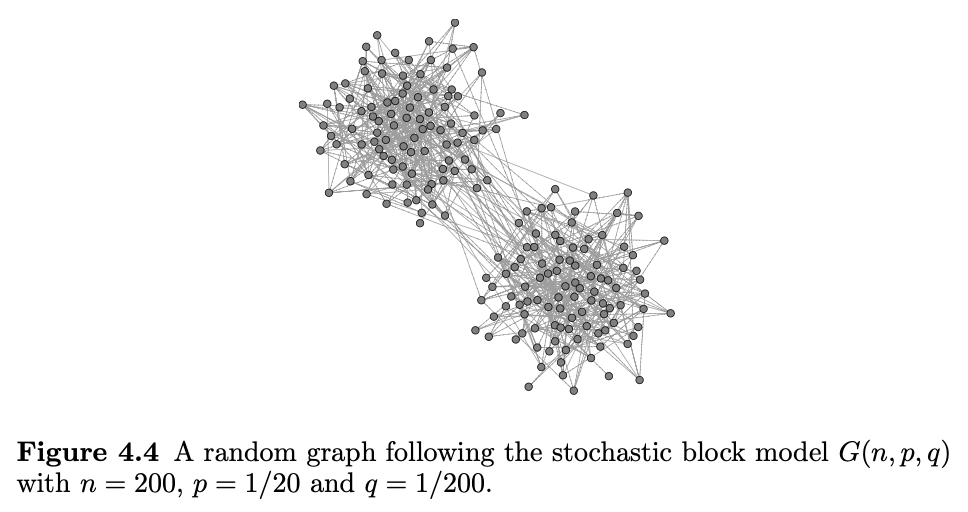
\includegraphics[width=0.8\textwidth]{Chapter 4/fig4-4.png}
\end{center}


\subsubsection{The Expected Adjacency Matrix Holds the Key}
A graph $G$ can be conveniently represented by its adjacency matrix $A$ (\cref{def:3.6.2}). For a random graph 
$G \sim G(n, p, q)$, the adjacency matrix $A$ is a random matrix, which we can use the tools we developed in 
this chapter to analyze.

Let's split $A$ into deterministic and random parts: 
\[ A = D + R \text{ where } D = \mathbb{E}\left[ A \right] \]
and think of $D$ as the \textit{signal} and R as \textit{noise}.

To see why $D$ is informative, let's compute its eigenstructure. The entries $A_{ij}$ have a Bernoulli 
distribution, either $\mathrm{Ber}(p)$ or $\mathrm{Ber}(q)$ depending on the community membership of vertices 
$i$ and $j$. So, the entries of $D$ are either $p$ or $q$, depending on the membership. For example, if we 
arrange vertices by community, then for $n = 4$, the matrix $D$ looks like this:
\[ D = \mathbb{E}\left[ A \right] = \begin{bmatrix}
p & p & q & q \\
p & p & q & q \\
q & q & p & p \\
q & q & p & p \\
\end{bmatrix}. \]
Take a look at the simpler matrix 
\[ \begin{bmatrix}
p & q \\
q & p \\
\end{bmatrix}. \]
Its eigenvalues are $\frac{p + q}{2}$ and $\frac{p - q}{2}$, with eigenvectors $(1, 1)^T$ and $(1, -1)^T$. 
The matrix $D$ is similar but with $p$ and $q$ replaced by $n/2 \times n/2$ blocks of the same values. So, $D$ 
also has rank 2, and its nonzero eigenvalues and eigenvectors are:
\[ \lambda_1(D) = \left( \frac{p + q}{2} \right)n, \ u_1(D) = \begin{bmatrix}
1 \\
\vdots \\
1 \\
-- \\
1 \\
\vdots \\
1 \\
\end{bmatrix}; \
\lambda_2(D) = \left( \frac{p - q}{2} \right)n, \ u_1(D) = \begin{bmatrix}
1 \\
\vdots \\
1 \\
-- \\
-1 \\
\vdots \\
-1 \\
\end{bmatrix}. \]
The key object here is the \textit{second} eigenvector of $u_2(D)$, which holds all the information about the 
community structure. If we know $u_2(D)$, we could identify the communities by the signs of its coefficients.


\subsubsection{The Actual Adjacency Matrix is a Good Approximation}
Unfortunately, we don't know the expected adjacency matrix $D = \mathbb{E}\left[ A \right]$. Instead, we know 
the actual adjacency matrix $A = D + R$, which is a noisy version of $D$. The level of the signal $D$ is 
\[ \lVert D \rVert_{} = \lambda_1 \asymp n \]
while the level of the noise $R$ can be estimated using \cref{cor:4.4.7}:
\[ \lVert R \rVert_{} \leq C \sqrt{n} \text{ with probability at least } 1 - 4e^{-n}. \]
So for large $n$, the noise $R$ is much smaller then the signal $D$. It means that $A$ is close to $D$, so we 
can just use the matrix $A$ instead of $D$ to extract the community inforemation. Let's justify this using the 
matrix perturbation theory developed earlier.


\subsubsection{Perturbation Theory}
We'll apply the David-Kahan inequality (\cref{thm:4.1.15}) to $D$ and $A$, focusing on the second largest 
eigenvalue. We need to check that $\lambda_2(D)$ is well-seperated from the rest of the spectrum of $D$, that 
is, from 0 and $\lambda_1(D)$. The distance is 
\[ \delta = \min_{}(\lambda_2(D), \lambda_1(D) - \lambda_2(D)) = \min_{}\left( \frac{p - q}{2}, q \right)n 
=: \mu n. \]
Recalling the bound on $R = A - D$, the Davis-Kahan inequality gives a bound on the angle between the 
\textit{unit} eigenvectors of $D$ and $A$ (indicated here by bars on top of the vectors):
\[ \sin{\angle (\bar{u_2}(D), \bar{u_2}(A))} \leq \frac{2 \lVert R \rVert_{}}{\delta} 
\lesssim \frac{\sqrt{n}}{\mu n} \lesssim \frac{1}{\mu \sqrt{n}}. \]
If the sine of the angle between two unit vectors is small, the vectors are close up to a sign (Exercise 4.16), 
so there exists $\theta \in \{ -1, 1 \}$ such that 
\[ \lVert \bar{u_2}(D) - \theta \bar{u_2}(A) \rVert_{2} \lesssim \frac{1}{\mu \sqrt{n}}. \]
We already computed the eigenvector $u_2(D)$ of $D$, but it was not a unit vector - it had norm $\sqrt{n}$. 
Multipkying both sides by $\sqrt{n}$, we get 
\[ \lVert u_2(D) - \theta u_2(A) \rVert_{2} \lesssim \frac{1}{\mu}. \]
This implies that the \textit{signs} of most coefficients of $u_2(D)$ and $\theta u_2(A)$ must agree. Indeed, 
rewriting the bound as 
\[ \sum_{j = 1}^{n}|u_2(D)_j - \theta u_2(A)_j|^2 \lesssim \frac{1}{\mu^2} \]
and noting that all coefficients of $u(D)$ are $\pm 1$, we see that each disagreement contributes between the 
signs of $u_2(D)_j$ and $\theta u_2(A)_j$ contributes at least 1 to the sum. Therefore, the number of 
disagreeing signs is $\lesssim \frac{1}{\mu^2}$.


\subsubsection{Spectral Clustering}
In summary, we use $u_2(A)$ to estimate $u_2(D)$, whose coefficients are $\pm 1$ and identify the two 
communities. This method for community detection is known as \textit{spectral clustering}:

\begin{algorithm}
	\caption{Spectral Clustering}
	\label{alg:sc}
	\begin{algorithmic}
		\item \textbf{Input:} graph $G$
		\item \textbf{Output:} a partition of the vertices $G$ into two communities
		\item \begin{enumerate}[label=\arabic*]
			\item Compute the adjacency matrix $A$ of the graph.
			\item Compute the eigenvector $v_2(A)$ for the second largest eigenvalue of $A$.
			\item Split vertices into two communities based on the signs of $v_2(A)$'s coefficients.
		\end{enumerate}
	\end{algorithmic}
\end{algorithm}

In fact, we have proved above that:
\begin{theorem}[Spectral clustering for the Stochastic Block Model]
\label{thm:4.5.2}
Let $G \sim G(n, p, q)$ and $\min_{}(q, p - q) = \mu > 0$. Then, with probability at least $1 - 4e^{-n}$, the 
spectral clustering algorithm identifies the communities of $G$ with at most $C / \mu^2$ misclassified 
vertices.
\end{theorem}

Summarizing, the spectral clustering algorithm correctly classifies all but $O(1)$ number of vertices, as long 
as the random graph is dense enough $(q \geq \text{const})$ and the probabilities of within- and across-
community edges are well seperated $(p - q \geq \text{const})$ . The condition $q \geq \text{const}$ is in fact 
not essential (Exercise 4.45).

\begin{remark}[Sparsity]
\label{rmk:4.5.3}
The sparsest graphs for which \cref{thm:4.5.2} is nontrivial, meaning $C / \mu^2 \leq n$, have expected average 
degree 
\[ \frac{n(p + q)}{2} \asymp \sqrt{n}. \]
With more tools, we will handle much more sparser graphs in Section 5.5.
\end{remark}



% ----------4.6----------
\subsection{Two-sided Bounds on Subgaussian Matrices}
\cref{thm:4.4.3} gives an upper bound on the singular values of an $\mathbb{R}^{m \times n}$ subgaussian 
random matrix $A$, which says 
\[ \sigma_1 \leq \lVert A \rVert_{} \leq C (\sqrt{m} + \sqrt{n}) \]
with high probability. 

In fact, there is a sharper two-sided bound on the \textbf{entire spectrum} of $A$:
\[ \sqrt{m} - C \sqrt{n} \leq \sigma_i \leq \sqrt{m} + C \sqrt{n}. \]
In other words, the below shows that a tall random matrix $\frac{1}{\sqrt{m}}A$ with $m \gg n$ is an 
approximate isometry.

\begin{theorem}[Name]
\label{thm:4.6.1}
Let $A \in \mathbb{R}^{m \times n}$ be a random matrix with independent, mean zero, subgaussian, isotropic 
tows $A_i$. Then for any $t \geq 0$ we have 
\[ \sqrt{m} - CK^2 (\sqrt{n} + t) \leq \sigma_n \leq \sigma_1 \leq \sqrt{m} + CK^2 (\sqrt{n} + t) \]
with probability at least $1 - 2 \exp{(-t^2)}$. Here $K = \max_{i} \lVert A_i \rVert_{\psi_2}$.
\end{theorem}

\begin{proof}
We'll prove a slightly stronger conclusion than the theorem statement, namely 
\[ \lVert \frac{1}{m}A^TA - I_n \rVert_{} \leq K^2 \max_{}(\delta, \delta^2) \text{ where } 
\delta = C \left( \sqrt{\frac{n}{m}} + \frac{t}{\sqrt{m}} \right). \]
Proving this implies proving the theorem (I haven't checked yet).

Again, we'll apply an $\varepsilon$-net argument, but use Bernstein inequality for the concentration step 
instead of Hoeffding which we did in \cref{thm:4.4.3}.

(\textbf{Approximation}) Using \cref{cor:4.2.11}, we can find an $\frac{1}{4}$-net $\mathcal{N}$ of the unit 
sphere $S^{n - 1}$ with cardinality 
\[ |\mathcal{N}| \leq 9^n. \]
Using \cref{lem:4.4.2}, we can evaluate the operator norm in the equation above on $\mathcal{N}$:
\[ \lVert \frac{1}{m}A^T A - I_n \rVert_{} \leq 2 \max_{x \in \mathcal{N}} 
\left| \left\langle (\frac{1}{m}A^T A - I_n)x, x \right\rangle \right| 
= 2 \max_{x \in \mathcal{N}} \left| \frac{1}{m} \lVert Ax \rVert_{2}^2 - 1 \right|. \]
Therefore, to prove the statement, it is enough to show that, with the required probability, 
\[ \max_{x \in \mathcal{N}} \left| \frac{1}{m} \lVert Ax \rVert_{2}^2 - 1 \right| \leq \frac{\varepsilon}{2} 
\text{ where } \varepsilon = K^2 \max_{}(\delta, \delta^2). \]

(\textbf{Concentration}) Fix $x \in \mathcal{N}$ and express $\lVert Ax \rVert_{2}^2$ as a sum of 
independent random variables: 
\[ \lVert Ax \rVert_{2}^2 = \sum_{i = 1}^{m} \left\langle A_i, x \right\rangle^2 =: \sum_{i = 1}^{m} X_i^2. \]
By assumption, the wors $A_i$ are independent, isotropic, and subgaussian random vectors with 
$\lVert A_i \rVert_{\psi_2} \leq K$. Thus $X_i = \left\langle A_i, x \right\rangle$ are independent subgaussian 
random variables with $\mathbb{E}[X_i^2] = 1$ and $\lVert X_i \rVert_{\psi_2} \leq K$. This makes 
$X_i^2 - 1$ independent, mean zero, and subexponential random variables with 
\[ \lVert X_i^2 - 1 \rVert_{\psi_1} \leq CK^2. \]
Thus we can use Bernstein inequality (\cref{cor:2.9.2}) and obtain 
\begin{align*}
	P \left( \left| \frac{1}{m}\lVert Ax \rVert_{2}^2 - 1 \right| \geq \frac{\varepsilon}{2} \right) 
	&= P \left( \left| \frac{1}{m} \sum_{i = 1}^{m} X_i^2 - 1 \right| \geq \frac{\varepsilon}{2} \right) \\
	&\leq 2 \exp{\left[ -c_1 \min_{}\left( \frac{\varepsilon^2}{K^4}, \frac{\varepsilon}{k^2} 
	\right)m \right]} \\
	&= 2 \exp{(-c_1 \delta^2 m)} \\
	&\leq 2 \exp{(-c_1 C^2(n + t^2))}.
\end{align*}
The last inequality comes from the definition of $\delta$ and using the inequality 
\[ (a + b)^2 \geq a^2 + b^2 \text{ for } a, b \geq 0. \]

(\textbf{Union bound}) Now unfix $x \in \mathcal{N}$. By union bound, 
\[ P \left( \max_{x \in \mathcal{N}} \left| \frac{1}{m}\lVert Ax \rVert_{2}^2 - 1 \right| 
\geq \frac{\varepsilon}{2} \right) 
\leq 9^n \cdot 2 \exp{(-c_1 C^2(n + t^2))} \leq 2 \exp{(-t^2)} \]
if we choose the constant $C$ to be large enough. Then by the necessary condition in the approximation step, 
the proof is complete.
\end{proof}

\begin{remark}[Expectation bound]
\label{rmk:4.6.2}
From \cref{rmk:4.4.4}, we can convert high-probability bounds to expectation bounds. Exercise 4.41 yields the 
following form for \cref{thm:4.6.1}:
\[ \mathbb{E}\left[ \lVert \frac{1}{m}A^T A - I_n \rVert_{} \right] \leq 
CK^2 \left( \sqrt{\frac{n}{m}} + \frac{n}{m} \right). \]
There is another version of the proof for \cref{thm:4.6.1} in Exercise 4.46.
\end{remark}



% ----------4.7----------
\subsection{Application: Covariance Estimation and Clustering}
When analyzing high-dimensional data, i.e. given points $X_1, \dots, X_m \in \mathbb{R}^n$ sampled from an 
unknown distribution, PCA is a basic way to analyze the data from Section 3.2.2.

PCA finds the ``principle components" as top eigenvectors of the data's covariance matrix. Although we do not 
know the covariance matrix of the underlying distribution, we can approximately estimate using the sample. The 
David-Kahan theorem (\cref{thm:4.1.15}) then helps us estimate the principle components of the underlying 
distribution.

How do we estimate the covariance matrix from the data? Let $X$ denote the random vector from the unknown 
distribution. For simplicity, assume $X$ has zero mean, and let's denote its covariance matrix by 
\[ \Sigma = \mathbb{E}\left[ XX^T \right]. \]
To estimate $\Sigma$, we can use the sample covariance matrix:
\[ \Sigma_m = \frac{1}{m}\sum_{i = 1}^{m}X_iX_i^T. \]
Since $X$ and $X_i$ are identically distributed, this estimate is unbiased:
\[ \mathbb{E}\left[ \Sigma_m \right] = \Sigma. \]
By the Law of Large Numbers (\cref{thm:1.7.1}) applied to each entry of $\Sigma$, we get 
\[ \Sigma_m \to \Sigma \text{ almost surely as } m \to \infty. \]
This leads to the quantitative problem: How big does the sample size $m$ need to be so that 
\[ \Sigma_m \approx \Sigma \text{ with high probability? } \]
For dimension reasons, we need at least $m \gtrsim n$ sample points. Let's show that $m \asymp n$ is enough.

\begin{theorem}[Covariance estimation]
\label{thm:4.7.1}
Let $X$ be a subgaussian random vector in $\mathbb{R}^n$. More speficically, assume that there exists 
$K \geq 1$ such that 
\[ \lVert \left\langle X, x \right\rangle \rVert_{\psi_2} \leq 
K \lVert \left\langle X, x \right\rangle \rVert_{L^2} = K x^T \Sigma x \text{ for any } x \in \mathbb{R}^n. \]
Then for every positive integer $m$, we have 
\[ \mathbb{E}\left[ \lVert \Sigma_m - \Sigma \rVert_{} \right] 
\leq CK^2 \left( \sqrt{\frac{n}{m}} + \frac{n}{m} \right) \lVert \Sigma \rVert_{}. \]
\end{theorem}

\begin{proof}
Let's first bring the random vectors $X, X_1, \dots, X_m$ to the isotropic position. For simplicity, assume 
that $\Sigma$ is invertible (This can be dropped like in Exercise 3.10). Setting 
\[ Z = Z_i = \Sigma^{-1/2}X, \]
then $Z, Z_1, \dots, Z_m$ are independent and isotropic random vectors satisfying 
\[ X = \Sigma^{1/2}Z \text{ and } X_i = \Sigma^{1/2} Z_i. \]
The assumption in the theorem then implies that (by \cref{def:3.4.1})
\begin{align*}
	\lVert Z \rVert_{\psi_2}^2 
	&= \sup_{s \in S^{n - 1}} \lVert \left\langle Z, x \right\rangle \rVert_{\psi_2}^2 \\
	&= \sup_{x \in S^{n - 1}} \lVert \left\langle \Sigma^{-1}X, x \right\rangle \rVert_{\psi_2}^2 \\
	&\leq \Sigma^{-1} \sup_{x \in S^{n - 1}} \lVert \left\langle X, x \right\rangle \rVert_{\psi_2}^2 \\
	&\leq K^2 \Sigma^{-1} \sup_{x \in S^{n - 1}} x^T \Sigma x \\
	&= K^2.
\end{align*}
Therefore $\lVert Z \rVert_{\psi_2} \leq K$ and $\lVert Z_i \rVert_{\psi_2} \leq K$. Then 
\[ \lVert \Sigma_m - \Sigma \rVert_{} = \lVert \Sigma^{1/2}R_m \Sigma^{1/2} \rVert_{} 
\leq \lVert R_m \rVert_{} \lVert \Sigma \rVert_{} \text{ where } 
R_m := \frac{1}{m}\sum_{i = 1}^{m}Z_iZ_i^T - I_n. \]
Consider the $m \times n$ random matrix $A$ whose rows are $Z_i^T$. Then 
\[ \frac{1}{m}A^T A - I_n = \frac{1}{m}\sum_{i = 1}^{m}Z_iZ_i^T - I_n = \mathbb{R}_m. \]
Applying \cref{thm:4.6.1}, we get 
\[ \mathbb{E}\left[ R_m \right] \leq CK^2 \left( \sqrt{\frac{n}{m}} + \frac{n}{m} \right) \]
(see \cref{rmk:4.6.2}). Substituting this into the bound for $\lVert \Sigma_m - \Sigma \rVert_{}$, we complete 
the proof.
\end{proof}

\begin{remark}[Sample complexity]
\label{rmk:4.7.2}
\cref{thm:4.7.1} shows that for any $\varepsilon \in (0, 1)$, we can estimate the covariance matric with a 
small relative error:
\[ \mathbb{E}\left[ \lVert \Sigma_m - \Sigma \rVert_{} \right] \leq \mathbb{E}\left[ \lVert \Sigma
\rVert_{} \right], \]
as long as the sample size is 
\[ m \asymp \varepsilon^{-2}n. \]
So, the sample covariance matrix gives a good estimate for the population covariance matrix \textit{if the 
sample size $m$ is proportional to the dimension $n$}.
\end{remark}

\begin{remark}[High-probability bound]
\label{rmk:4.7.3}
Out argument also gives a high-probability bound: for any $u \geq 0$, we have 
\[ \lVert \Sigma_m - \Sigma \rVert_{} \leq 
CK^2 \left( \sqrt{\frac{n + u}{m}} + \frac{n + u}{m} \right) \lVert \Sigma \rVert_{} \]
with probability at least $1 - 2e^{-u}$. See Exercise 4.49.
\end{remark}


\subsubsection{Application: Clustering of Point Sets}
Let's illustrate \cref{thm:4.7.1} with an application to clustering. In particular, we'll do this for Gaussian 
mixture models (GMMs):

\begin{definition}[]
\label{def:4.7.4}
Generate $m$ random points in $\mathbb{R}^n$ like this. Flip a fair coin; if it comes up heads, draw a point 
from $N(\mu, I_n)$, and if it comes up tails, from $N(-\mu, I_n)$. This distribution is called the 
\underline{Gaussian mixture model} with means $\pm \mu$.
\end{definition}

Equivalently, consider a random vector 
\[ X = \theta \mu + g \]
where $\theta$ is a Rademacher random variable, $g \sim N(0, I_n)$, and $\theta$ and $g$ are independent. 
Draw a sample $X_1, \dots, X_m$ of independent random vectors identically distributed with $X$. Then the sample 
is distributed according to the Gaussian mixture model; See Figure 4.5.

\begin{center}
	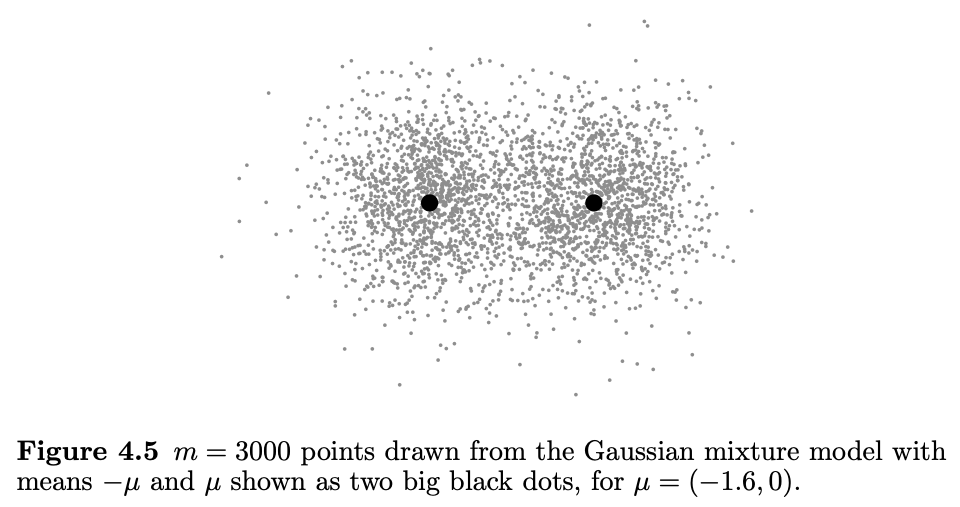
\includegraphics[width=0.8\textwidth]{Chapter 4/fig4-5.png}
\end{center}

Given $m$ sample points from a Gaussian mixture model, we would like to know which points belong to which 
cluster. To do this, we can use a variant of the \textit{spectral clustering} algorithm.

To see why a spectral method might work here, notice that the distribution of $X$ is not isotropic, but rather 
stretched along $\mu$ (the horizontal direction in Figure 4.5). Thus, we can approximately find $\mu$ by 
computing the first principal component of the data via PCA. Next, we can project the data points onto the 
principle component and classify them based on which side of the origin they lie on. Here is the algorithm:

\begin{algorithm*}
	\caption{Spectral Clustering for GMMs}
	\label{alg:scgmm}
	\begin{algorithmic}
		\item \textbf{Input:} points $X_1, \dots, X_m \in \mathbb{R}^n$
		\item \textbf{Output:} a partition of the points into two clusters 
		\item \begin{enumerate}[label=\arabic*]
			\item Compute the sample covariance matrix $\Sigma_m = \frac{1}{m}\sum_{i = 1}^{m}X_iX_i^T$.
			\item Compute the top eigenvector $v = v_1(\Sigma_m)$.
			\item Split the points $X_i$ into two communities based on the sign of $\left\langle X_i, v
			\right\rangle$.
		\end{enumerate}
	\end{algorithmic}
\end{algorithm*}

\begin{theorem}[Spectral clustering for GMMs]
\label{thm:4.7.5}
Take points $X_1, \dots, X_m \in \mathbb{R}^n$ from the Gaussian mixture model with means $\pm \mu$. If 
$m \geq Cn$ and $\lVert \mu \rVert_{2} \geq C$, then with probability at least 0.99, the spectral clustering 
algorithm identifies the communities, with at most 1\% of misclassified points.
\end{theorem}

\begin{proof}
Exercise 4.51.
\end{proof}

It is remarkable that accurate classification is possible even when the cluster seperation $\lVert \mu 
\rVert_{2}$ is much smaller than their diameter, which is $\asymp \sqrt{n}$.

